\documentclass{article}

\usepackage{graphicx}
\usepackage{tikz}
\usepackage{tikzsymbols}
\usetikzlibrary{calc,patterns,shapes.geometric}
\pagestyle{empty}
\usepackage[margin=0pt]{geometry}
\geometry{papersize={14in,12in}}

\def\centerarc[#1](#2)(#3:#4:#5){\draw[#1] ($(#2)+({#5*cos(#3)},{#5*sin(#3)})$) arc (#3:#4:#5);}

\begin{document}
	\begin{figure}
		\centering
		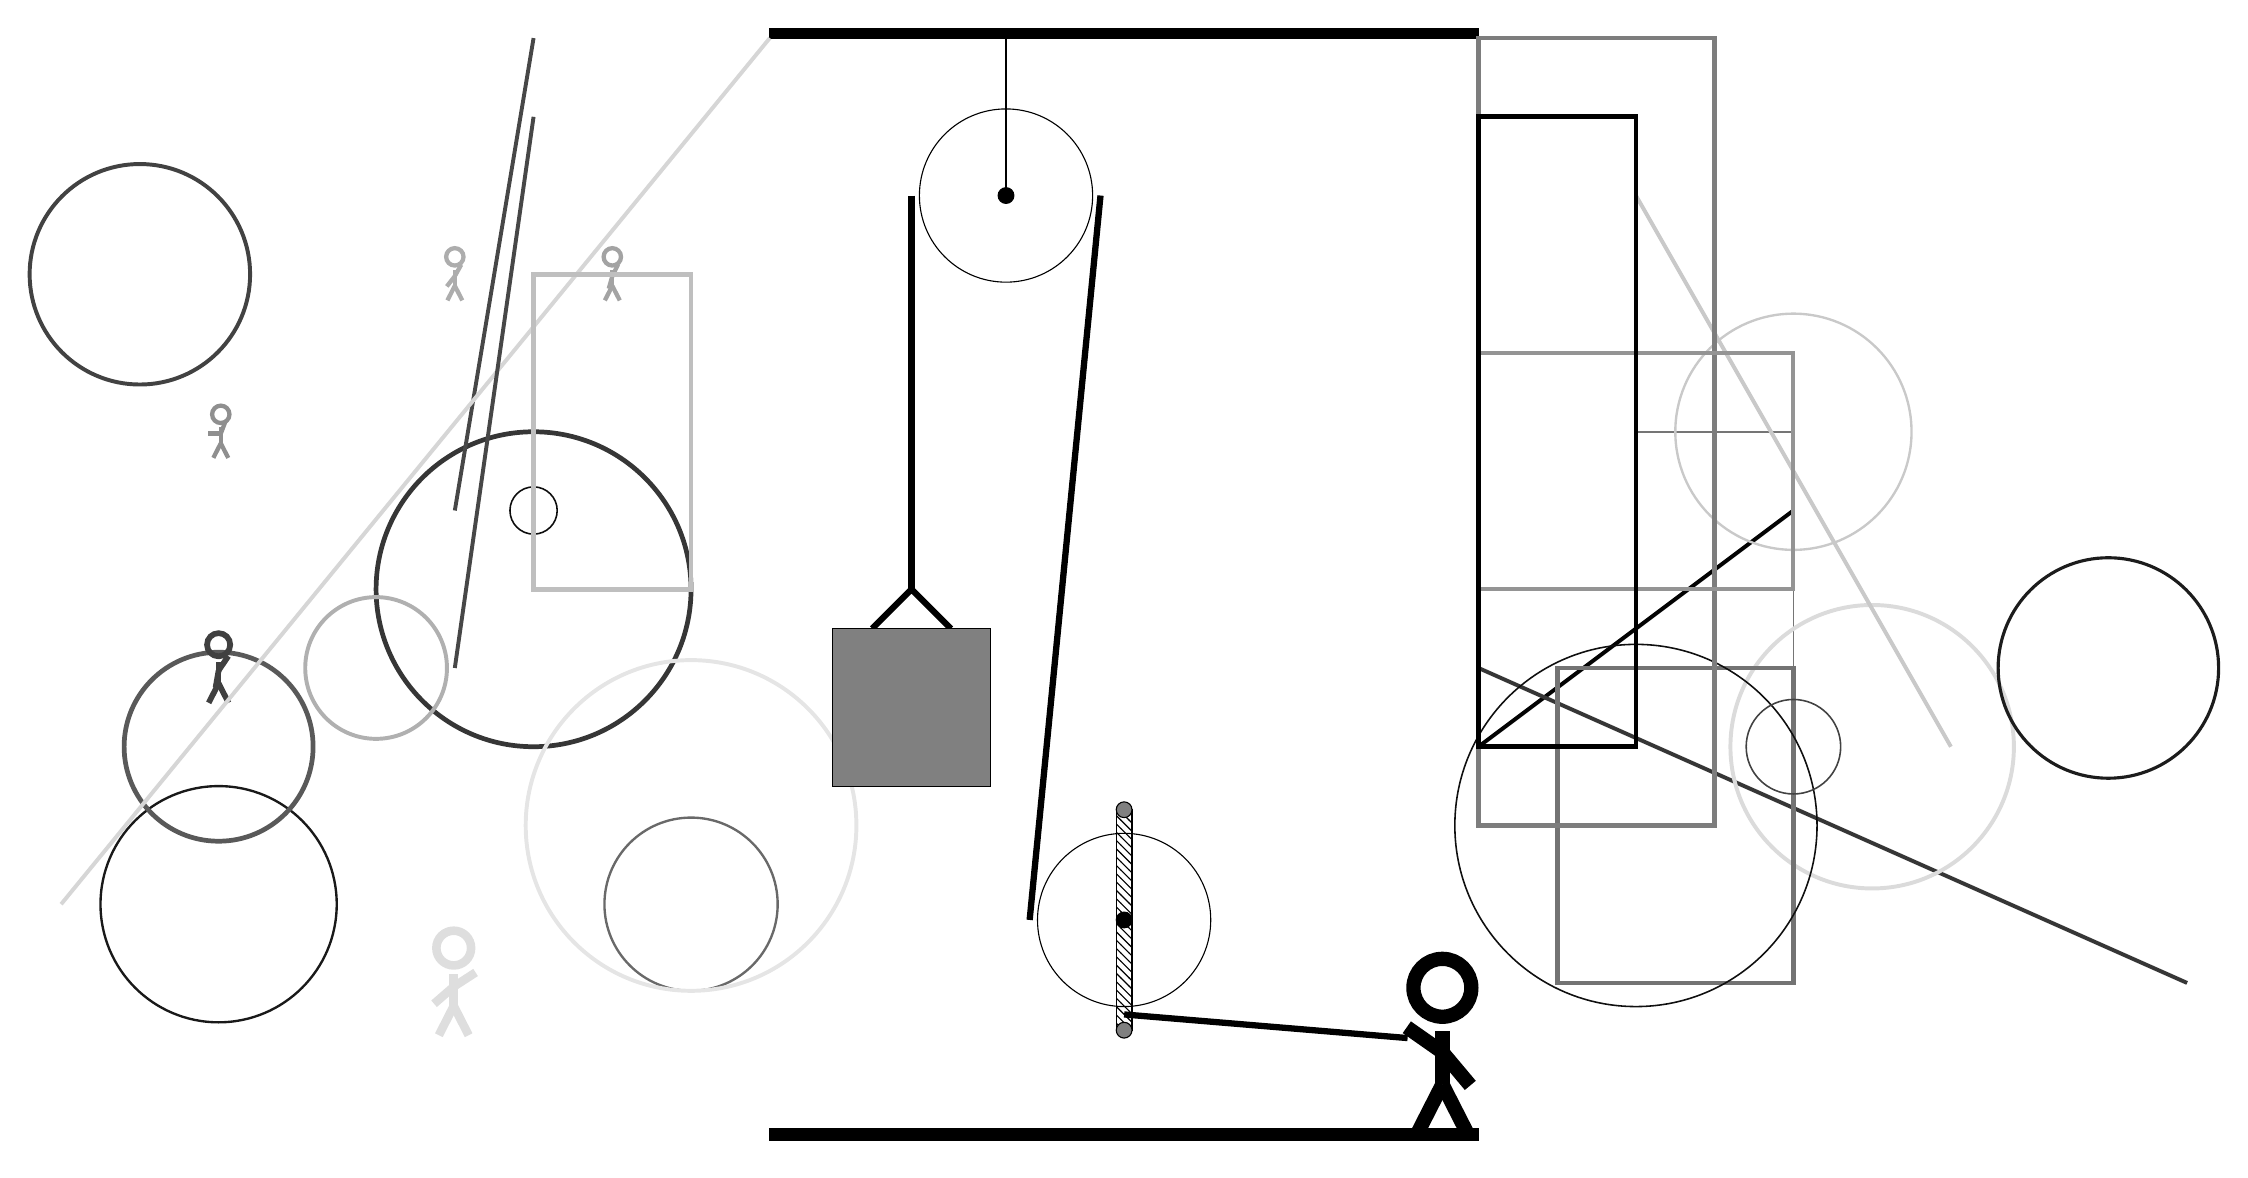
\begin{tikzpicture}
			%%%%% START %%%%%
			
			\draw[fill=black] (-2, 14) rectangle (7, 14.125);
			
			\draw (1, 12) circle (1.1);
			\draw[fill=black] (1, 12) circle (0.1);
			\draw (1, 14) -- (1, 12);
			
			\draw[fill=white](2.5, 2.8) circle (1.1);
			\draw[fill=black] (2.5, 2.8) circle (0.1);
			\draw[pattern=north west lines, pattern color=black] (2.4, 4.2) rectangle (2.6, 1.4);
			\draw[fill=black!50] (2.5, 4.2) circle (0.1);
			\draw[fill=black!50] (2.5, 1.4) circle (0.1);
			
			\draw[line width=0.5mm, color=black!99](11, 8) -- (7, 5);
			
			\draw [line width=0.6mm, color=black!79](-5, 7) circle (2.0);
			\draw[line width=0.5mm, color=black!79](7, 6) -- (16, 2);
			\node[line width=0.6mm, color=black!36] at (-4, 11) {\Strichmaxerl[3][74][64]};
			
			\node[line width=0.7mm, color=black!32] at (-6, 11) {\Strichmaxerl[3][52][61]};
			\draw[line width=0.2mm, color=black!54] (9, 9) rectangle (11, 6);
			\draw [line width=0.5mm, color=black!14](12, 5) circle (1.8);
			\draw [line width=0.2mm, color=black!95](-5, 8) circle (0.3);
			\node[line width=0.4mm, color=black!44] at (-9, 9) {\Strichmaxerl[3][0][69]};
			\draw[line width=0.5mm, color=black!72](-6, 8) -- (-5, 14);
			\node[line width=0.3mm, color=black!13] at (-6, 2) {\Strichmaxerl[6][41][33]};
			\draw[line width=0.6mm, color=black!55] (8, 2) rectangle (11, 6);
			\draw[line width=0.5mm, color=black!21](9, 12) -- (13, 5);
			\draw [line width=0.2mm, color=black!94](9, 4) circle (2.3);
			\draw [line width=0.2mm, color=black!74](11, 5) circle (0.6);
			\draw [line width=0.3mm, color=black!90](-9, 3) circle (1.5);
			
			\draw [line width=0.6mm, color=black!65](-9, 5) circle (1.2);
			
			\draw [line width=0.3mm, color=black!21](11, 9) circle (1.5);
			\draw [line width=0.4mm, color=black!89](15, 6) circle (1.4);
			
			\node[line width=0.3mm, color=black!75] at (-9, 6) {\Strichmaxerl[4][80][56]};
			\draw [line width=0.5mm, color=black!74](-10, 11) circle (1.4);
			
			\draw[line width=0.6mm, color=black!51] (7, 4) rectangle (10, 14);
			\draw[line width=0.5mm, color=black!16](-2, 14) -- (-11, 3);
			\draw[line width=0.6mm, color=black!25] (-3, 11) rectangle (-5, 7);
			\draw[line width=0.5mm, color=black!72](-5, 13) -- (-6, 6);
			
			\draw [line width=0.3mm, color=black!59](-3, 3) circle (1.1);
			
			\draw[line width=0.5mm, color=black!42] (7, 10) rectangle (11, 7);
			\draw [line width=0.5mm, color=black!31](-7, 6) circle (0.9);
			\draw[line width=0.6mm, color=black!100] (7, 13) rectangle (9, 5);
			
			\draw [line width=0.5mm, color=black!10](-3, 4) circle (2.1);
			
			\draw[line width=0.8mm] (-0.7, 6.5) -- (-0.2, 7.0) -- (0.3, 6.5);
			\draw[fill=black!50] (-1.2, 6.5) rectangle (0.8, 4.5);
			
			\draw[line width=0.8mm] (-0.2, 12) -- (-0.2, 7.0);
			\centerarc[line width=0.8mm](1, 12)(0:180:1.2000000000000002);
			\draw[line width=0.8mm](2.2, 12) -- (1.3, 2.8);
			\centerarc[line width=0.8mm](2.5, 2.8)(180:270:1.2000000000000002);
			\draw[line width=0.8mm](2.5, 1.6) -- (6.1, 1.3);
			
			\node at (6.5, 1.2) {\Strichmaxerl[10][-35][-50]};
			
			\draw[fill=black] (-2, 0) rectangle (7, 0.15);
			
			%%%%% END %%%%%
		\end{tikzpicture}
	\end{figure}	
\end{document}